\only<beamer>{\titleframe}

\begin{frame}{Overview}
    \tableofcontents
\end{frame}


\section{Introduction}
\begin{frame}{What are Cellular Automata?}
    \begin{itemize}
        \item Discrete models: grid of cells, each with a state
        \item Simple, local rules $\rightarrow$ complex global behavior
        \item Used for simulating complex systems (urban, physics, biology)
        \item Example: Conway's Game of Life
    \end{itemize}
\end{frame}


\section{1D Cellular Automata}
\begin{frame}{1D Cellular Automata: Theory}
    \begin{itemize}
        \item Cells in a 1D array, each with a state (e.g., 0 or 1)
        \item Neighborhood: e.g. cell itself + left/right neighbors
        \item Update rules: Neighborhood $\rightarrow$ next state
    \end{itemize}
\end{frame}

\begin{frame}{1D CA: Ruleset}
    \begin{figure}
        \centering
        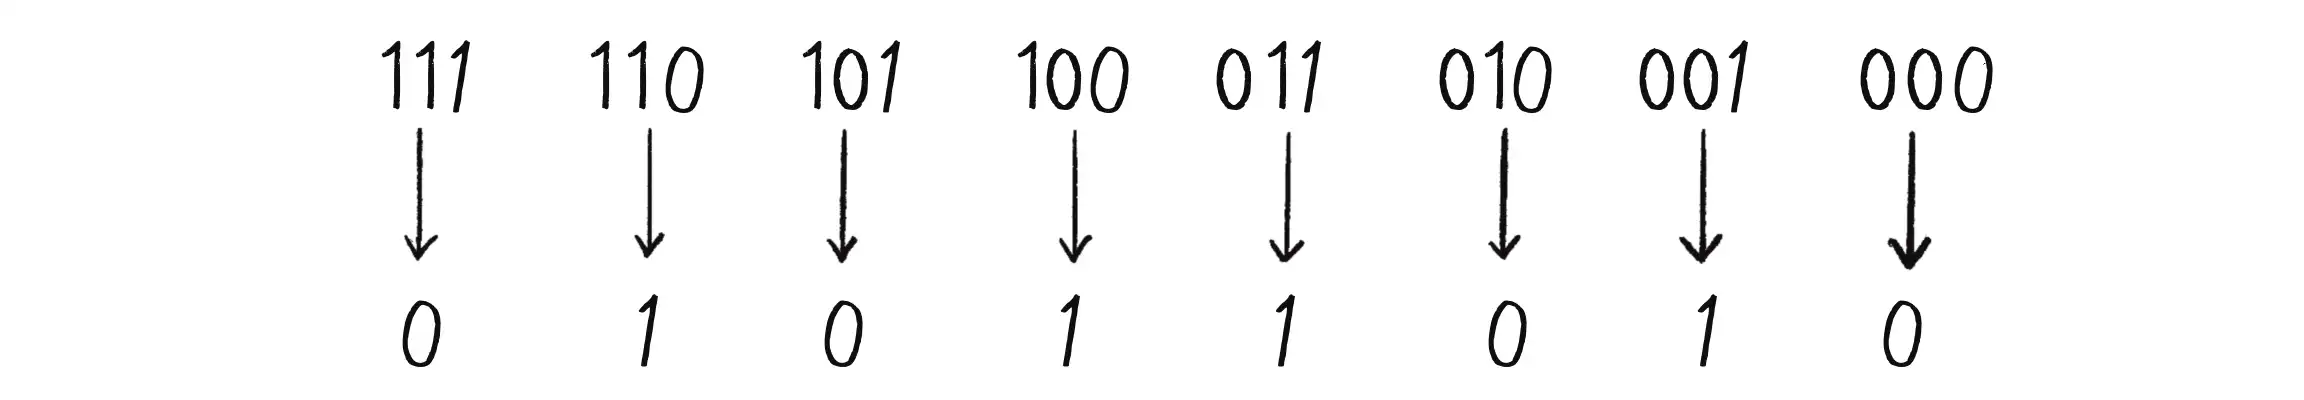
\includegraphics[width=\textwidth]{../paper/figures/ruleset_example.png}
        \caption{Example: Mapping neighborhood to next state (here rule number 90)}
    \end{figure}
\end{frame}

\begin{frame}{1D CA: Visualization}
    \begin{figure}
        \centering
        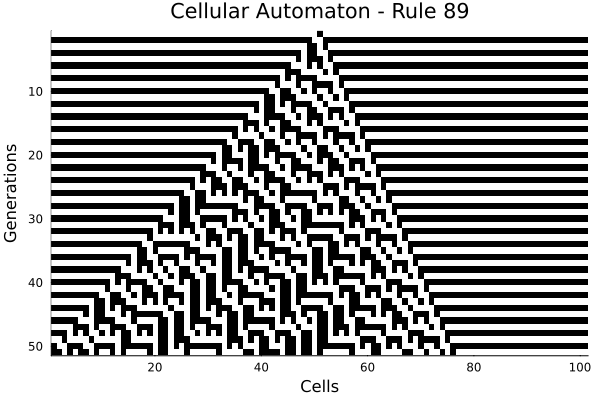
\includegraphics[width=0.5\textwidth]{../paper/figures/carule89}
        \caption{Visualization of generations as rows in a 2D grid}

    \end{figure}

\end{frame}


\section{Wolfram Classification}
\begin{frame}{Wolfram Classification}
    \begin{columns}
        \column{0.4\linewidth}
        \begin{itemize}
            \item \textbf{Class 1:} Uniformity (stable)
            \item \textbf{Class 2:} Repetition (periodic)
            \item \textbf{Class 3:} Random (chaotic)
            \item \textbf{Class 4:} Complexity (mix of order/chaos)
        \end{itemize}
        \column{0.6\linewidth}
        \begin{figure}
            \centering
            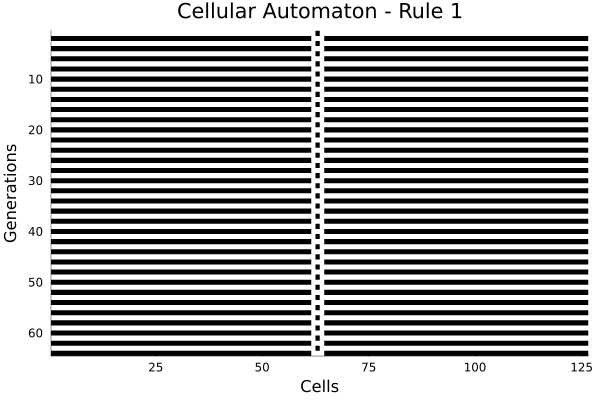
\includegraphics[width=0.8\textwidth]{../paper/figures/rule1.png}
            \caption{Rule 1: An example of Class 2 (repetitive)}
        \end{figure}
    \end{columns}
\end{frame}


\section{2D Cellular Automata}
\begin{frame}{2D Cellular Automata: Game of Life}
    \begin{columns}
        \column{0.4\linewidth}
        \begin{itemize}
            \item Grid of cells, each with $8$ neighbors
            \item \textbf{Rules:}
                  \begin{itemize}
                      \item Birth: exactly $3$ alive neighbors
                      \item Survival: $2$ or $3$ alive neighbors
                      \item Death: $<2$ or $>3$ alive neighbors
                  \end{itemize}
        \end{itemize}
        \column{0.6\linewidth}
        \begin{figure}
            \centering
            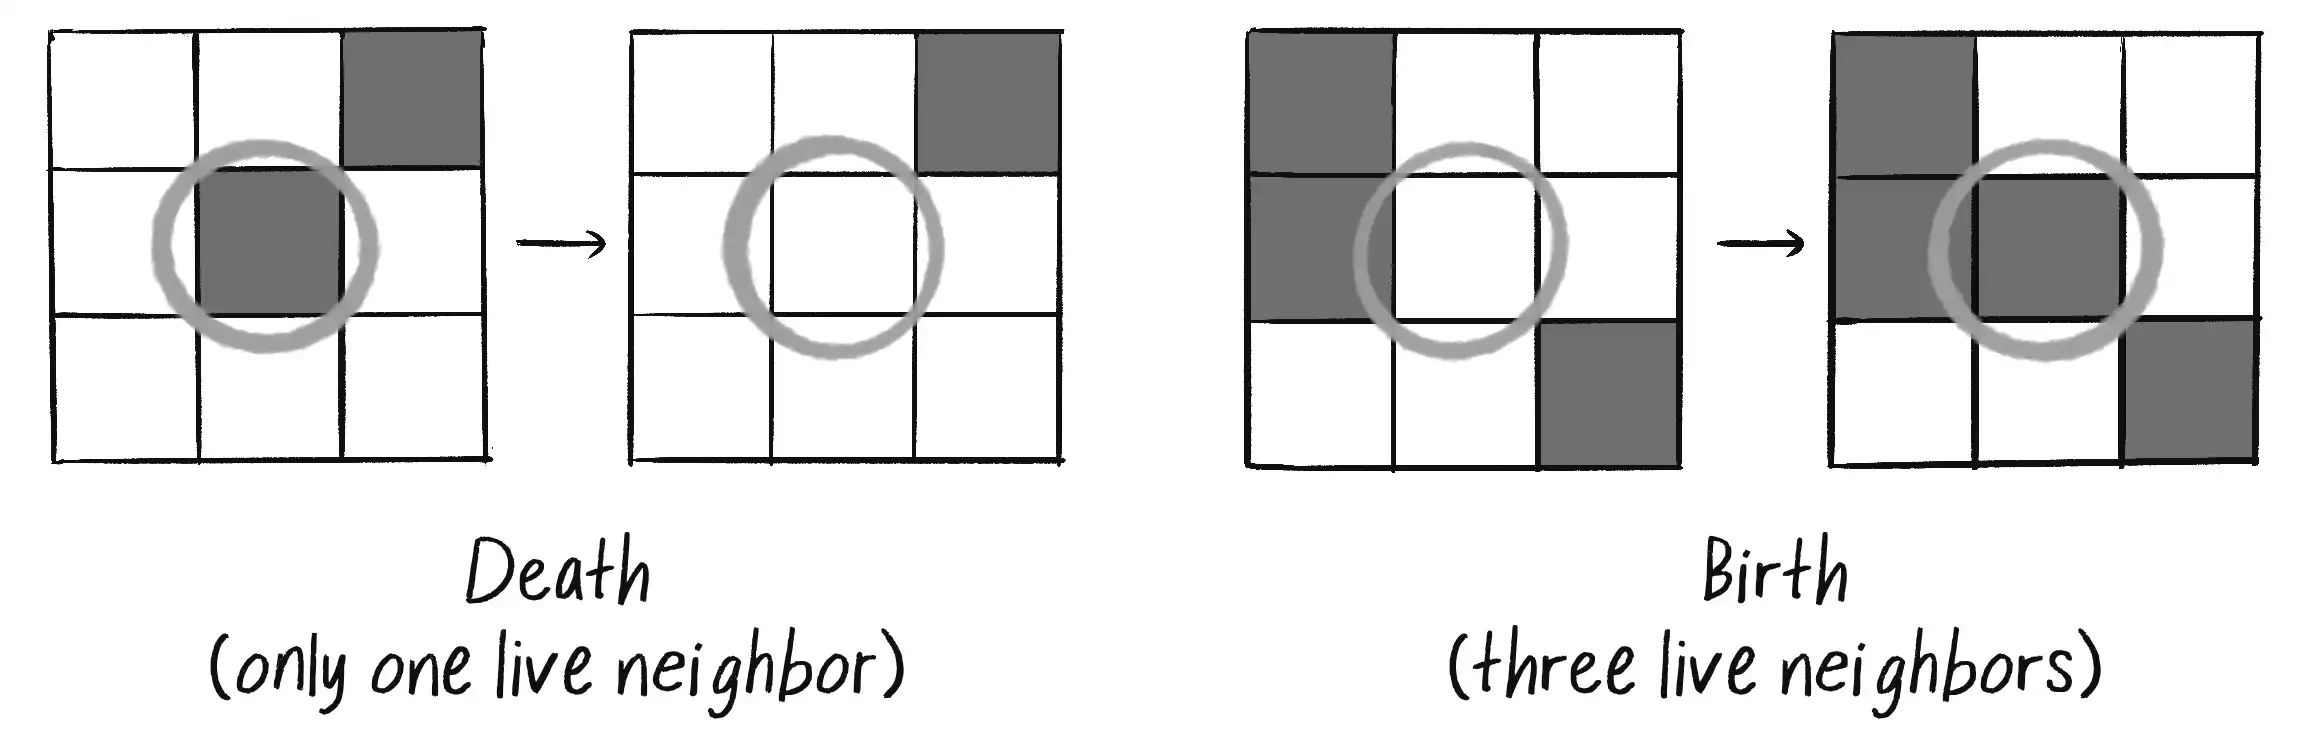
\includegraphics[width=\textwidth]{../paper/figures/game_of_life_examples}
            \caption{Examples of scenarios in the Game of Life, Source: \url{https://natureofcode.com/static/99dd5b32b72ce094d5a77f749c2ab9f0/3ca65/07_ca_28.webp}}
        \end{figure}
    \end{columns}

\end{frame}

\begin{frame}{Game of Life: Patterns}
    \begin{columns}
        \column{0.4\linewidth}
        \begin{itemize}
            \item \textbf{Stable:} Do not change
            \item \textbf{Oscillators:} Repeat after $n$ steps
            \item \textbf{Spaceships:} Move across grid
            \item \textbf{Guns:} Emit other patterns
        \end{itemize}
        \column{0.6\linewidth}
        \centering
        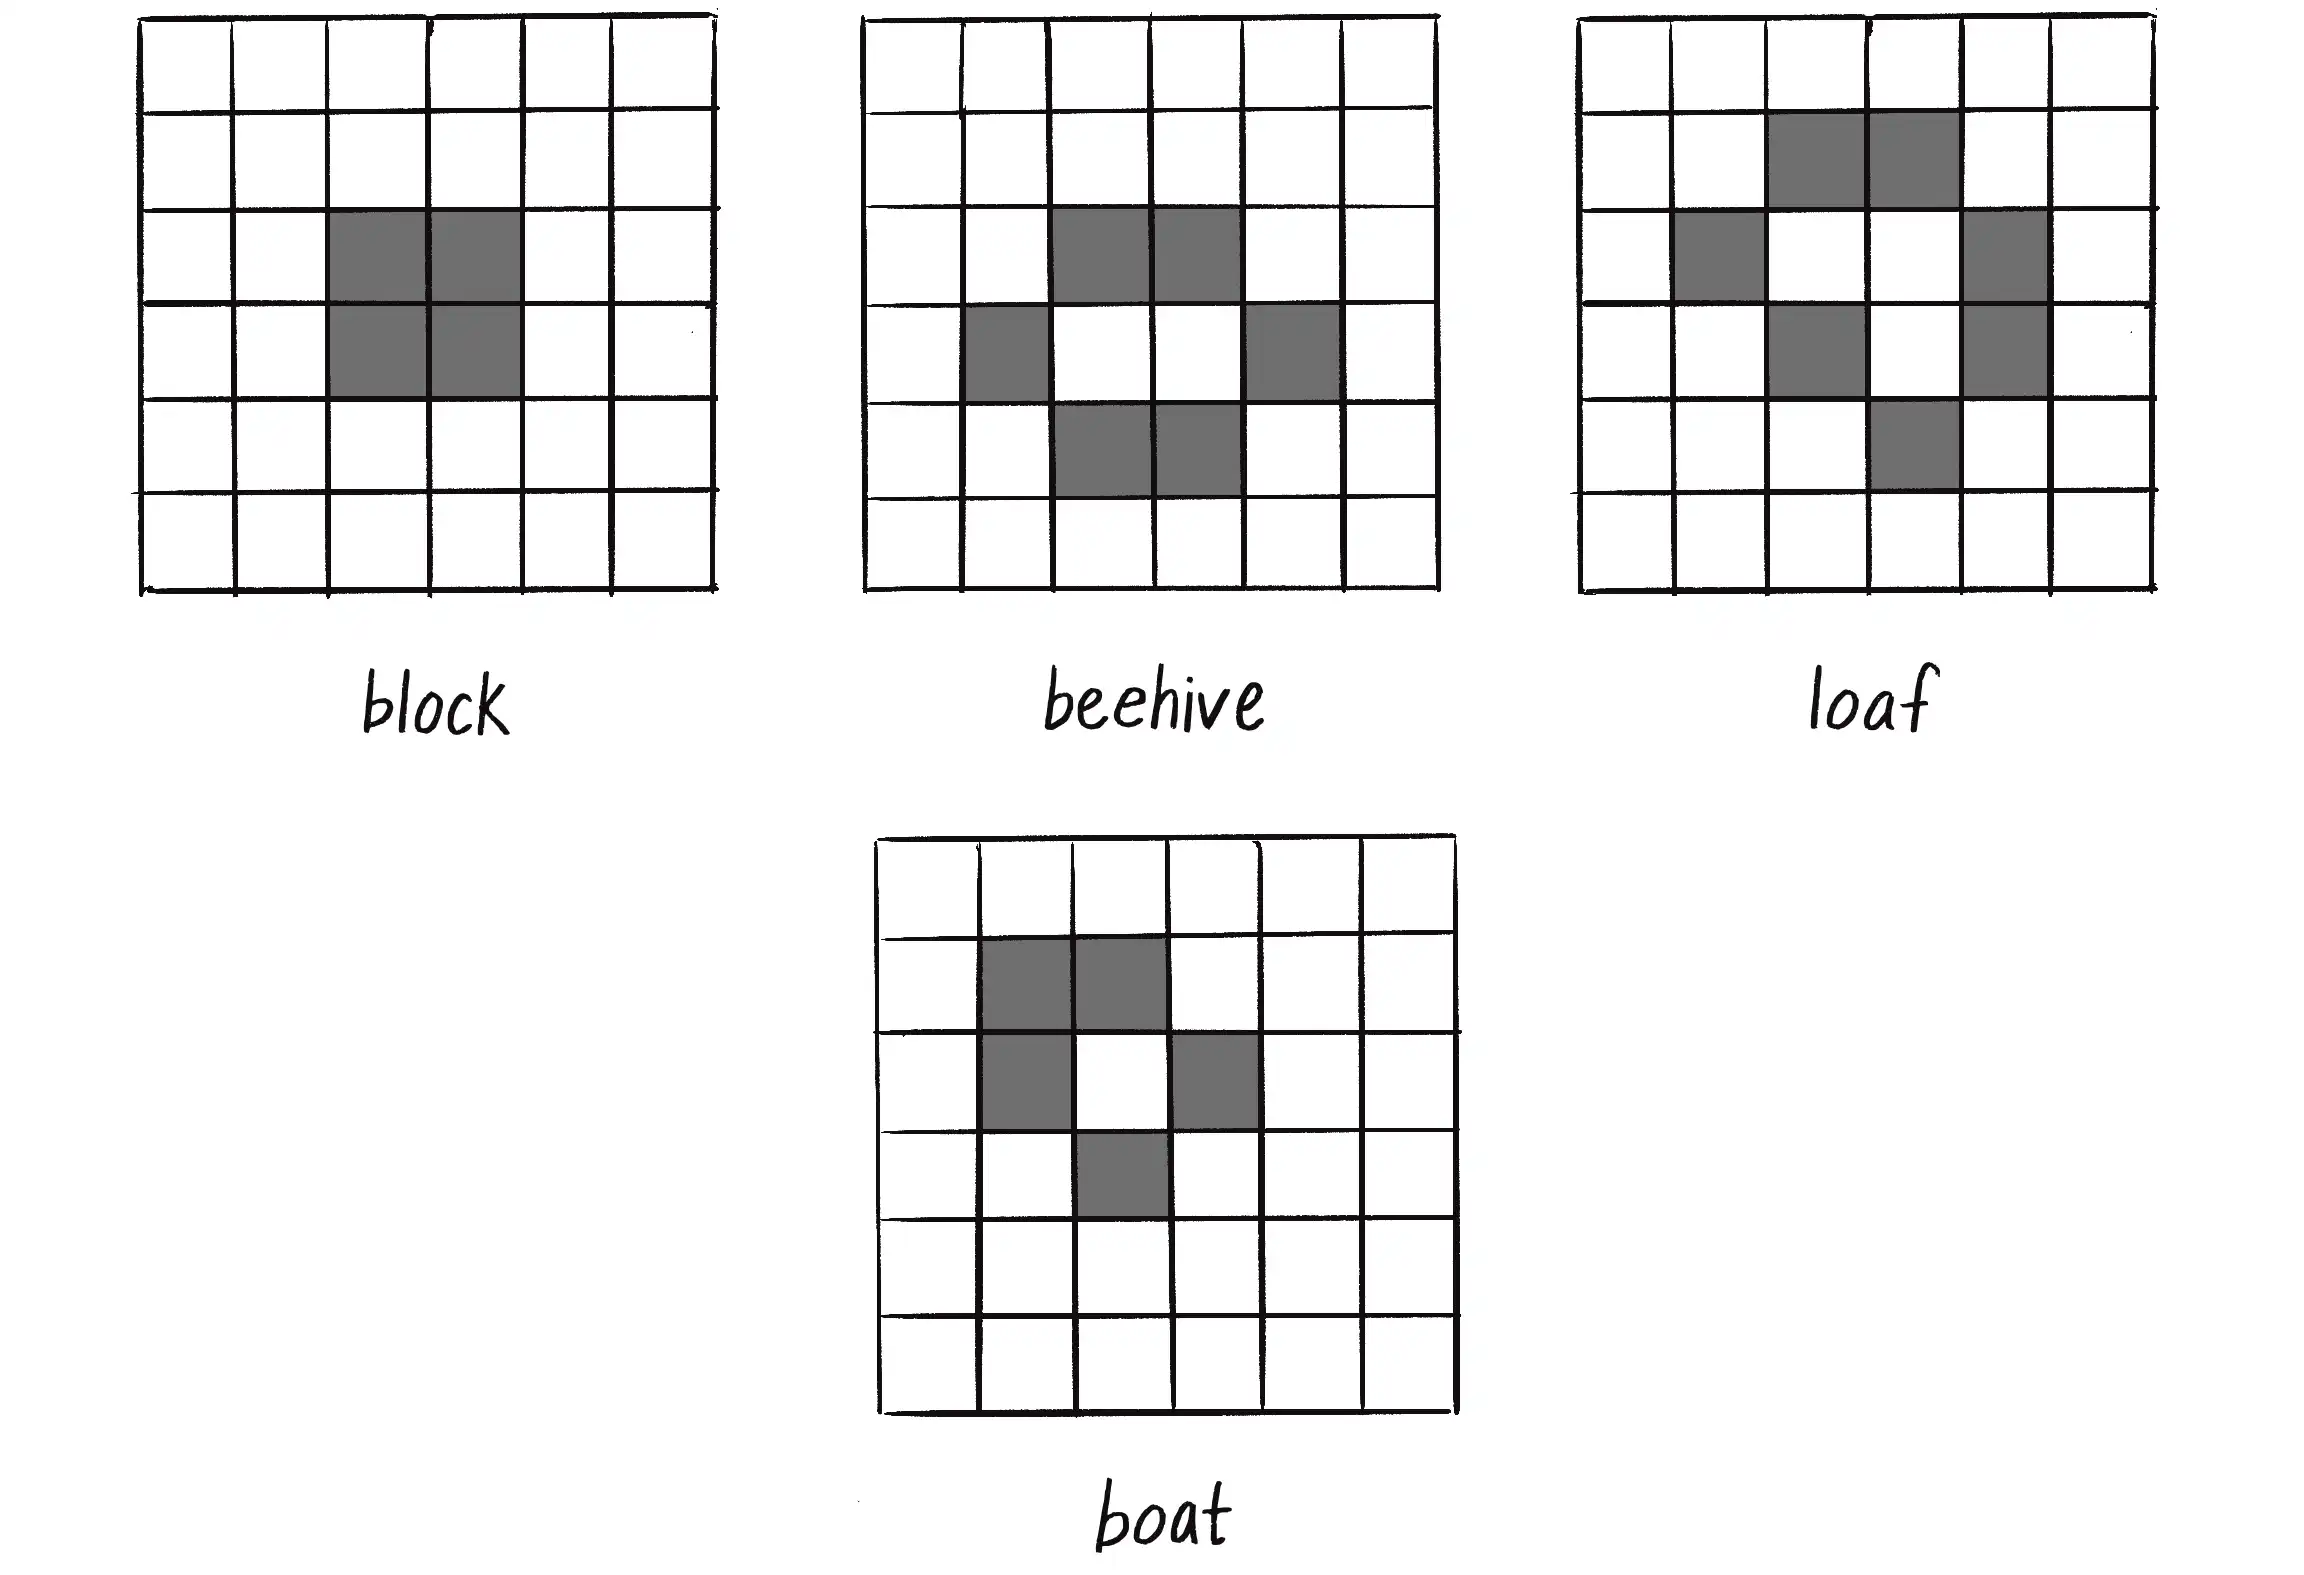
\includegraphics[height=8em]{../paper/figures/stable}\\
        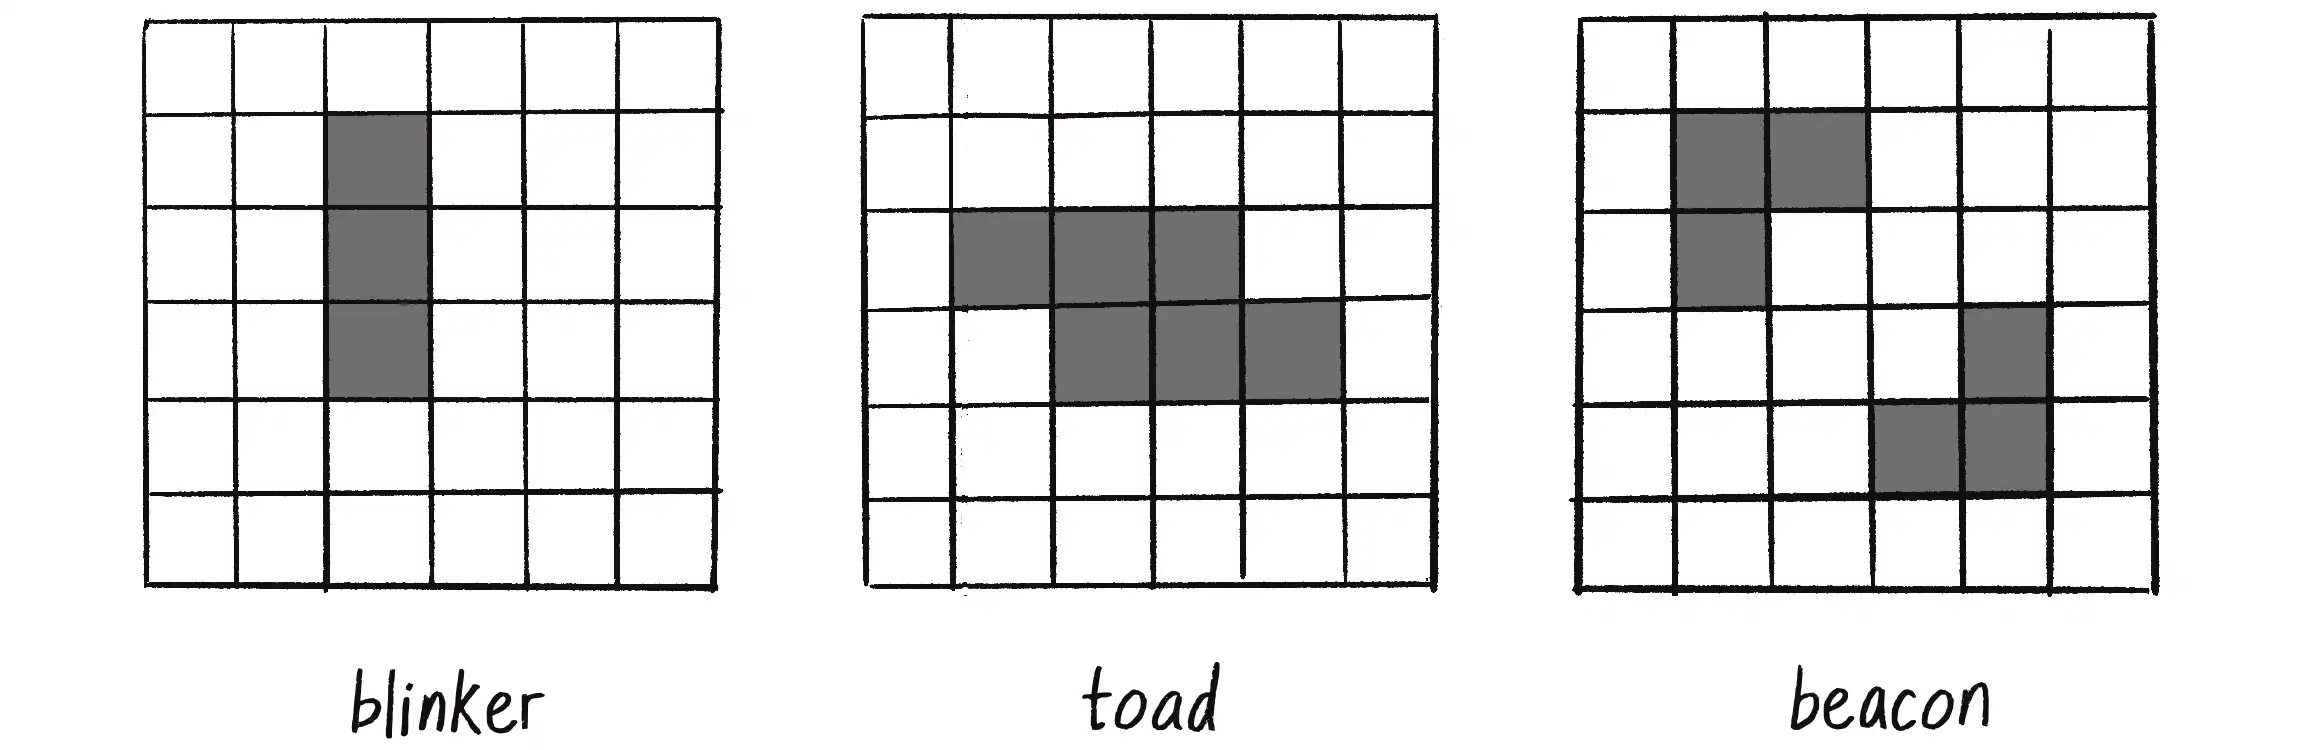
\includegraphics[height=5em]{../paper/figures/oscillator}\\
        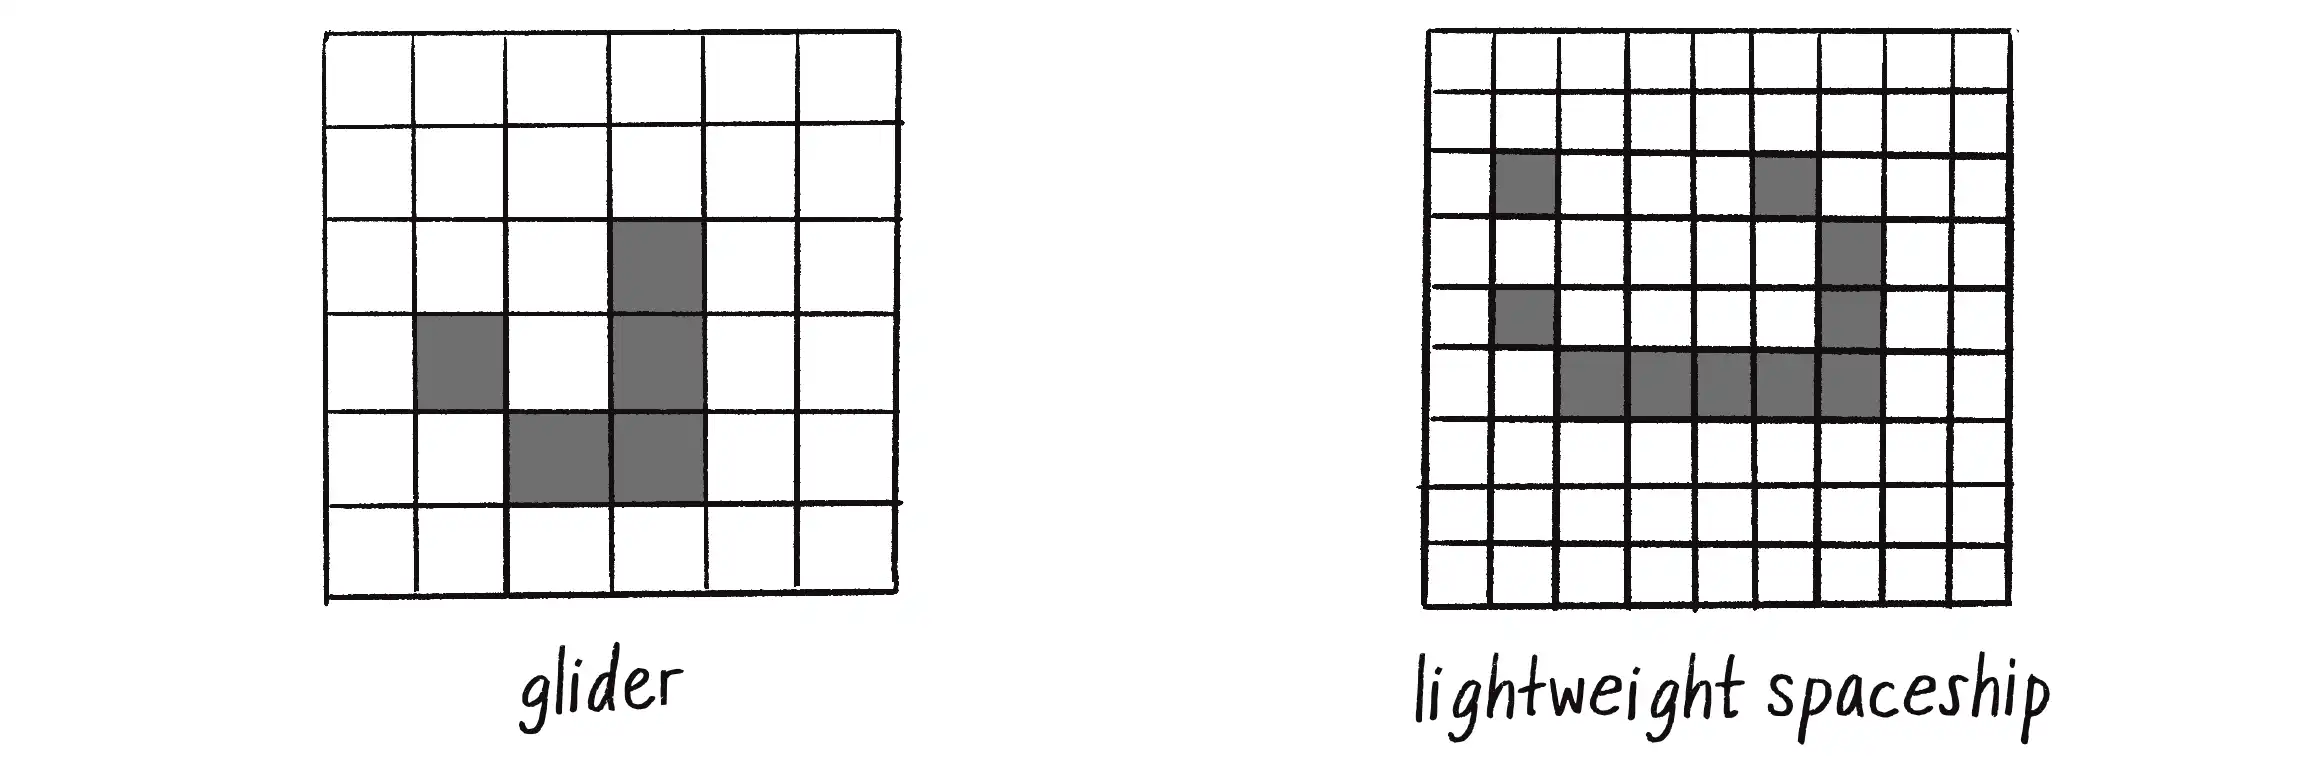
\includegraphics[height=5em]{../paper/figures/spaceship}

    \end{columns}
\end{frame}


\section{Implementation in Julia}
\begin{frame}{1D CA in Julia}

\end{frame}

\begin{frame}{Game of Life in Julia}

\end{frame}

\begin{frame}{Extending Game of Life: Infection Simulation}

\end{frame}


\section{Julia vs. Other Languages}
\begin{frame}{Why Julia for Simulation?}

\end{frame}


\section{Discussion}
\begin{frame}{Discussion}

\end{frame}


\section{Conclusions}
\begin{frame}{Conclusions}

\end{frame}

\begin{frame}{Image sources}

\end{frame}


\begin{frame}{Thanks / References}

\end{frame}
